\documentclass[
    11pt,
]{article}

\usepackage{authblk}

% \usepackage{natbib}
% \setcitestyle{nature}

\usepackage[style=nature, natbib]{biblatex}

\addbibresource{References.bib}

\RequirePackage{luatex85, shellesc} % work around the LuaTex bug
% options for packages which may be loaded elsewhere
\PassOptionsToPackage{unicode=true, pdfa}{hyperref}
\PassOptionsToPackage{hyphens}{url}
\PassOptionsToPackage{dvipsnames,svgnames*,x11names*}{xcolor}

%==============================================================================%
%                                Load packages                                 %
%==============================================================================%

\usepackage{amsmath}                  % the AMS Math package - provides useful math environments and tools

\usepackage{amssymb}                  % provides useful symbols

\usepackage{amsfonts}                 % provides nice mathematical fonts

\usepackage{bm}                       % bold math

\usepackage{calc}                     % gives the ability to calculate in the document itself, inferior to but lighter weight than pythontex

\usepackage{cancel}                   % provides environments to cancel stuff in mathmode

\usepackage{esint}                    % better and more integral signs

\usepackage{enumitem}                 % enumerate and itemize improvements

\usepackage{fancyhdr}                 % fancy headers and footers

\usepackage[vario]{fancyref}          % for fancy cross-referencing with vario-style refs

\usepackage{graphicx}                 % facilitates inclusion of external graphics

\usepackage{parskip}                  % produces zero \parindent and non-zero \parskip

\usepackage{setspace}                 % set space between lines

\usepackage{xcolor}                   % colours bro

\usepackage{unicode-math}             % allows unicode characters in mathmode

\usepackage[pdfa, unicode]{hyperref}  % hyperlinks and PDF metadata manipulation

\usepackage{tikz}                     % drawing

\usepackage[siunitx]{circuitikz}      % drawing circuits

\usepackage{pgfplots}                 % plotting

\usepackage{geometry}                 % to set the margins of the page

\usepackage{subfig}

%==============================================================================%
%                             Set package options                              %
%==============================================================================%

%============================%
%          AMSMath           %
%============================%

\allowdisplaybreaks

%============================%
%          Hyperref          %
%============================%

\hypersetup{
    pdftitle={A minimal reaction-diffusion neural model generates C. elegans undulation},
    pdfauthor={Anshul Singhvi},
    colorlinks=true,
    linkcolor=Maroon,
    citecolor=Blue,
    urlcolor=Blue,
    breaklinks=true,
    pdfdisplaydoctitle = true
}

%============================%
%         Microtype          %
%============================%

% \UseMicrotypeSet[protrusion]{basicmath} % disable protrusion for tt fonts

%============================%
%     TikZ and PGFPlots      %
%============================%

\usetikzlibrary{
    arrows.meta,
    calc,
    decorations,
    decorations.pathreplacing,
    decorations.footprints,
    math,
    patterns,
    shadows,
    external
}

\tikzset{>=stealth}

\pgfplotsset{compat=1.16}

\usepgfplotslibrary{
    polar,
    colormaps,
    colorbrewer,
    groupplots,
    statistics
}

% This cycle list encodes the Wong colors, which are visually distinguishable.
% They also account for colorblind support, and as such are optimal for use in a paper.
\pgfplotscreateplotcyclelist{wong}{%
    color={rgb, 255 : red, 86  ; green, 180 ; blue, 233}, mark = *\\         % sky blue
    color={rgb, 255 : red, 230 ; green, 159 ; blue, 0},   mark = square*\\   % orange
    color={rgb, 255 : red, 0   ; green, 158 ; blue, 115}, mark = otimes*\\   % blueish green
    color={rgb, 255 : red, 240 ; green, 228 ; blue, 66},  mark = star\\      % yellow
    color={rgb, 255 : red, 0   ; green, 114 ; blue, 178}, mark = diamond*\\  % blue
    color={rgb, 255 : red, 213 ; green, 94  ; blue, 0},   mark = triangle*\\ % vermillion
    color={rgb, 255 : red, 204 ; green, 121 ; blue, 167}, mark = pentagon*\\ % reddish purple
}

\pgfplotsset{every axis legend/.append style={%
        cells={anchor=west}
    },
    cycle list name = wong,
}

%============================%
%          Geometry          %
%============================%

\geometry{
  a4paper,
  margin = 1.2in
}

%==============================================================================%
%                         Macros and document options                          %
%==============================================================================%

\setstretch{1} % line spacing of 1.25

\setlength{\emergencystretch}{3em}  % prevent overfull lines
\providecommand{\tightlist}{%
  \setlength{\itemsep}{0pt}\setlength{\parskip}{0pt}}
% \setcounter{secnumdepth}{0}
%
% % Redefines (sub)paragraphs to behave more like sections
% \ifx\paragraph\undefined\else
%     \let\oldparagraph\paragraph
%     \renewcommand{\paragraph}[1]{\oldparagraph{#1}\mbox{}}
% \fi
% \ifx\subparagraph\undefined\else
%     \let\oldsubparagraph\subparagraph
%     \renewcommand{\subparagraph}[1]{\oldsubparagraph{#1}\mbox{}}
% \fi

\newcommand{\inputtikz}[1]{%
  \tikzsetnextfilename{#1}%
  \input{#1.tikz}%
}

%==============================================================================%
%                            Neuron diagram macros                             %
%==============================================================================%

\newcommand{\doublec}[2]{% double diffusion arrows
  \draw  [-Circle] ($(#1.north east)!0.7!(#1.north)$) -- ($(#2.south east)!0.7!(#2.south)$);
  \draw  [Circle-] ($(#1.north west)!0.7!(#1.north)$) -- ($(#2.south west)!0.7!(#2.south)$);
  }

\newcommand{\singlec}[2]{% single diffusion arrows
  \draw [-Latex] (#1.east) -- (#2.west);
  }

% Set the TikZ neuron style up, since it's used many times
\tikzset{
  neuron/.style={
  % The shape:
  circle,
  % The size:
  minimum size=6mm,
  % The border:
  very thick,
  draw=blue!50!black!50,
  % The filling:
  top color=white,
  bottom color=blue!50!black!20, % and something else at the bottom
  % Font
  font=\itshape,
  % padding around node
  outer sep=2mm
  }
}


\tikzexternalize

\begin{document}
% \sffamily

%==============================================================================%
%                              Title and abstract                              %
%==============================================================================%

\title{A minimal reaction-diffusion neural model generates {\emph{C. elegans}} undulation}

\author[1]{Anshul Singhvi}

\author[1,3]{Harold Hastings}

\author[2]{Jenny Magnes}

\author[2]{Cheris Congo}

\author[2]{Miranda Hulsey-Vincent}

\author[2]{Susannah Zhang} 

\author[1]{Rifah Tasnim}

\author[1]{Naol Negassa}

\affil[1]{Bard College at Simon's Rock}
\affil[2]{Vassar College}
\affil[3]{Hofstra University}

\date{\today}

\begin{abstract}
    % Note: this is project https://www.overleaf.com/project/5e984f87a777200001dcff7e

    The small (1 mm) nematode \emph{Caenorhabditis elegans} (see wormbook.org) has become widely used as a model organism; in particular the \emph{C. elegans} connectome has been completely mapped, and \emph{C. elegans} locomotion has been widely studied (\citet{corsi2015}). We describe a minimal reaction-diffusion model for the locomotion of \emph{C. elegans}, using as a framework a simplified version of Xu et al.'s "descending pathway" description of the \emph{C. elegans} central pattern generator (CPG) \citet{xu2018,wen2012}.  Finally, we realize a model of the required oscillations and coupling with a network of coupled \citet{keener1983} analog neurons.
    We note that \citet{olivares2019} present a likely more realistic model which relies on small networks of neurons, and presents a distributed model of the CPG. We use the simpler simulation to show that a small network of \citet{fitzhugh1955}-\citet{nagumo1962} neurons (one of the simplest neuronal models) can generate key features of \emph{C. elegans} undulation (see \citet{magnes2012}), and thus locomotion.
\end{abstract}

\maketitle

\section{Introduction}\label{sec: intro}

The small (1 mm) nematode \emph{Caenorhabditis elegans} (\emph{C. elegans}) has become a widely used model organism (cf. http://www.wormbook.org \cite{corsi2015}), and has been among the most studied biological models of neuronal development and locomotion \citep{katz2016, corsi2015}.
The \emph{C. elegans} connectome has been completely mapped \citep{jabr} and, as described below, its locomotion has been widely studied (\citet{corsi2015, gjorgjieva2014, }).  There are a variety of neuronal models which can generate such undulation,
``When crawling on a solid surface, the nematode C. elegans moves forward by propagating sinusoidal dorso-ventral retrograde contraction waves.  A uniform propagating wave leads to motion that undulates about a straight line.'' \citep{kim2011}.
A different type of locomotion, often called swimming, occurs when nematodes are submerged in a liquid medium. The nematodes “switch” between these two gaits, by changing the dynamics of the CPG.

The purpose of this paper is to describe a minimal, biomimetic, reaction-diffusion model for the \emph{C. elegans} central pattern generator (CPG) \citep{xu2018, wen2012}.  We use simulation methods to show that a small network of \citet{fitzhugh1955}-\citet{nagumo1962} neurons (one of the simplest neuronal models) based on a skeleton model of the \emph{C. elegans} CPG can reproduce key features of \emph{C. elegans} undulation \citep{magnes2012} and thus locomotion.

Finally, we describe an analog electronic implementation of our model through solving a modified version of the FitzHugh-Nagumo neuron \cite{fitzhugh1955}, based upon an analog circuit originally proposed by \citet{keener1983}.  This circuit solves the Keener differential equations, and we adjusted it to allow diffusive coupling between neurons.  We constructed a small network with these ``neuro-mimetic'' circuits, and showed that their behaviour replicates FitzHugh-Nagumo simulated behaviour.

There are many other models for the CPG; for example, a 2019 preprint by \cite{olivares2019} proposes a distributed network of self-oscillating systems of neurons, instead of a structured chain like our proposed CPG.  The point of this paper is to create a minimal working model, though, and not to strive for full realism.  Our CPG model can be interpreted as having a graph-like structure, and it is easy to manipulate the "weights" of the edges (connections between neurons) of this "graph" to study defects or other changes in the CPG in an efficient, reproducible and explainable way.  Additionally, the simplicity of the model means that it is easy, given a set of parameters, to investigate and reason about the reason for some behaviour of a worm.  Since conditions in the lab are not exactly controllable, our model allows for the

\citet{olivares2019} recently created a more biologically relevant model for the CPG, which argues that the CPG is a network of connected, self-oscillating systems.  The role of this paper is to show a very minimal model, and our approach has been to create a small and computationally cheap model.

\section{The model central pattern generator}

% TODO show how the latest paper describes a small sequence of neurons forming coupled oscillators.

A central pattern generator is a small neural circuit which generates and regulates the movement of complex organisms.  This structure is present in different forms in many animals, and it regulates many types of periodic motion.  \citet{xu2018} proposed an architecture for the CPG of \emph{C. elegans} which is described below in \fref{fig: xu_cpg}.

In more complex animals, like horses or dogs, there is only one CPG; the dynamics of the CPG change depending on the gait of the animal \citep{collins1994}.  The mode of locomotion depends on the sequence in which the neurons fire, but the network's topology remains the same.  We show later that breaking the symmetry of the CPG model can lead to radical changes in behaviour.
\setcounter{figure}{1}
\begin{figure}[h!]
    % begin a continued float; see
    % https://tex.stackexchange.com/questions/118192/figure-subnumbering-1a
    \ContinuedFloat*
    \centering
    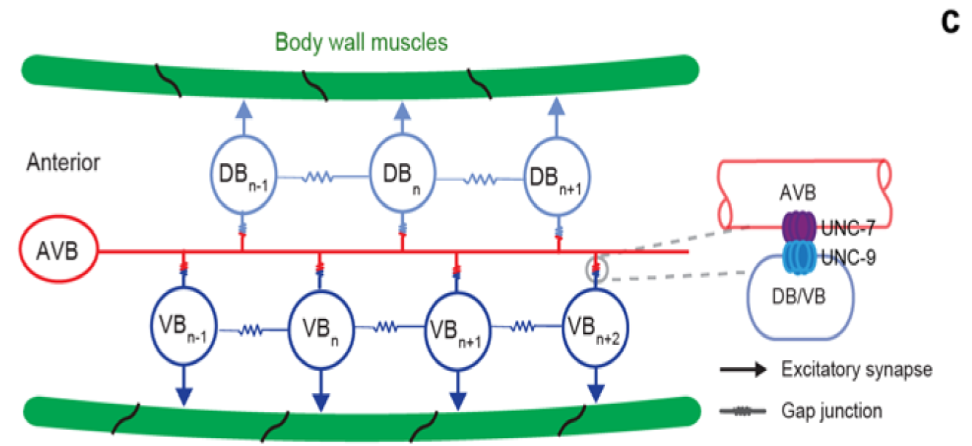
\includegraphics[width=9cm]{figures/xu_cpg/xu_cpg.png}
    \caption{The central pattern generator proposed by \citet{xu2018}.  Note the structure of the neurons, especially the head oscillator driving the descending pathway.}
    \label{fig: xu_cpg}
\end{figure}

The simple model \emph{C. elegans} central pattern generator which is used here has two principal components.  First is the \textbf{head oscillator}. As described by \citet{gjorgjieva2014}, the head oscillator consists of two “head neurons” with mutually inhibitory coupling. Oscillations are generated when this coupling destabilizes an excitable steady state.

In the terms of dynamical systems analysis, the oscillations destabilize to a stable limit cycle.  The mutual inhibition and symmetry between neuron pairs leads to a phase lock of $180^\circ$.  This provides out-of-phase stimuli which propagate through the descending pathway, with the inhibition between neuron pairs keeping the oscillations stable.

Second is the \textbf{descending pathway}, which consists of pairs of coupled, excitable, dorsal and ventral neurons.  These follow the body of the worm, and are linked to motor neurons and muscles. The head oscillator drives the descending pathway, and the pathway is kept in sync by mutual inhibitory coupling between neurons.

% TODO expand.  Our model could have had more neurons, with a shorter phase lag between pairs.
Although \emph{C. elegans} has twelve pairs of motor neurons, we have only used six pairs in our model.  An equivalent result could be obtained with more neurons, by increasing the coefficient of diffusion along the pathway, causing a shorter phase lag between neuron pairs.  \Fref{fig: cpg} is a depiction of our simplified model as a graph, wherein neurons are nodes, and the arrows between them symbolize connections.

\begin{figure}[h!]
    % continue the previous continued float
    \ContinuedFloat
    \centering
    \inputtikz{figures/cpg/cpg}
    \caption{Our simplified central pattern generator model, based upon the descending pathway of Xu. The model includes inhibitory connections between corresponding dorsal and ventral neurons (denoted by subscripts $d$ and $v$, respectively) and a descending pathway of gap junctions.}
    \label{fig: cpg}
\end{figure} % TODO: legend

\section{The FitzHugh-Nagumo Neuronal Model}\label{sec: fhn}

As described above, we sought the simplest relevant neuronal model.  The classical Hodgkin-Huxley\cite{hodgkin1952} model of squid neurons has led to a variety of simpler conduction models, including the Morris-Lecar\cite{morris1981} and Fitzhugh-Nagumo (FHN) models.

The FHN model consists of two dynamical variables; a fast activator variable $v$ corresponding to the (rescaled) membrane potential, and a slow inhibitor variable $w$ corresponding to a generalized gating variable.

\begin{equation}
    \label{eq: fhn}
    \begin{aligned}
        \frac{dv}{dt} &= f(v) + w + I_\mathrm{ext}\\
        \frac{dw}{dt} &= \varepsilon(v - \gamma w + \alpha)\\
        f(v) &= \frac{v^3}{3} - v
    \end{aligned}
\end{equation}

The parameter $I_\mathrm{ext}$ is an external driving current, and is used here to model the effect of gap junctions and synapses upon membrane potential.  The parameter $\alpha$ determines the vertical position of the $w$-nullcline and thus controls excitability. Action potentials can also be generated by a current injection corresponding to $I_\mathrm{ext}$. Finally, the parameter $\varepsilon$ determines ratio between the time scales of the fast activator variable $v$ and the slow inhibitor variable $w$; $\gamma$ limits the growth of $w$.

In addition, $f(v)$ can be any function which retains the appropriate dynamics, in that it has the same general shape as the cubic $f(v) = \frac{v^3}{3} - v$.  For example, $f(v)$ could be replaced by the cubic-like I-V curve of the tunnel diode in the \citet{nagumo1962} circuit, or even the piecewise linear approximation generated in the \citet{keener1983} circuit used in our implementation.

\citet{xu2018} described a simplified two-variable model consisting of a fast, cubic-like activator variable (see the V-nullcline) and a slow, non-linear inhibitor variable (see the n-nullcline). The \citet{xu2018} neuronal model can thus be interpreted as a Fitzhugh-Nagumo type model neuron.

% remark that if the w and v nullclines come near each other, you see a critical slowdown.
% In Hodgkin-Huxley notation, $n$ is the potassium channel.  In the FHN formulation, this corresponds to the $w$ gate variable.
\begin{figure}[h!]
    \label{fig: nm nullclines}
    \centering
    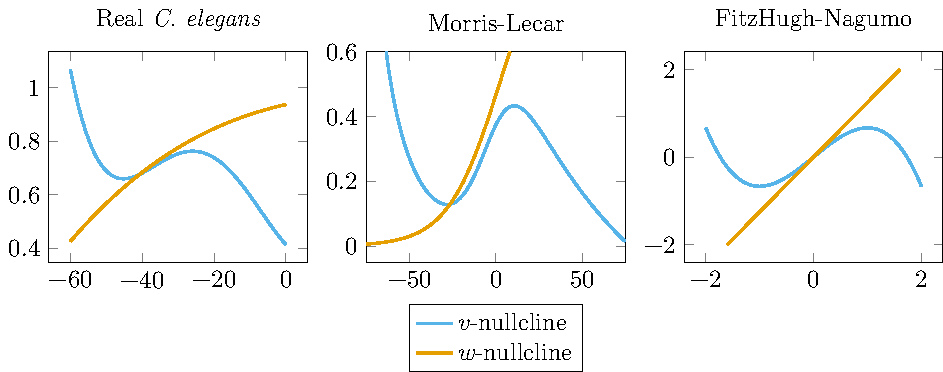
\includegraphics{figures/neuron_dynamics/neuron_dynamics.pdf}
    % note that in the vicinity of the v-nullcline, the w-nullcline is essentially straight.
    \caption{Dynamics of \textit{C. elegans} neurons following Xu \textit{et al.} \cite{xu2018} (left) and Fitzhugh-Nagumo neurons \cite{fitzhugh1955, nagumo1962} (right).}
\end{figure}

% TODO: see if anyone else used diffusion to couple neurons
 Following *** references are Collins and Richmond which you have and Yanagita T, Ichinomiya T, Oyama Y. Pair of excitable Fitzhugh-Nagumo elements: Synchronization, multistability, and chaos. Physical Review E. 2005 Nov 28;72(5):056218. , we now use
generalized diffusion coupling between FHN neurons to model gap junctions and synapses. The effect of gap junctions and synapses upon the membrane potential is modeled by replacing the external current $I_\mathrm{ext}$ of the system, by a generalized diffusion term, $D \max(Δv,0)$. A positive diffusion coefficient $D$ is used to simulate a gap junction, or an excitatory synapse and a negative coefficient to simulate an inhibitory synapse (\citet{collins1994}).

% TODO: there will be other examples...cf them

This yields the the system of (modified) FitzHugh-Nagumo equations:

\begin{equation}
    \label{eq: fhnd}
    \begin{aligned}
        \frac{dv}{dt}   &= f(v) + w  + \color{black}{D(Δv)}\\
        \frac{dw}{dt}   &= \varepsilon (v - \gamma w + \alpha)\\
        f(v) &= \frac{v^3}{3} - v
    \end{aligned}
\end{equation}

where $\Delta v$ is the difference in voltage between the driving and driven neurons, essentially $\Delta v = v_{driven} - v_{driving}$.


\begin{figure}[h!]
    \label{fig: fhn_dynamics}
    \centering
    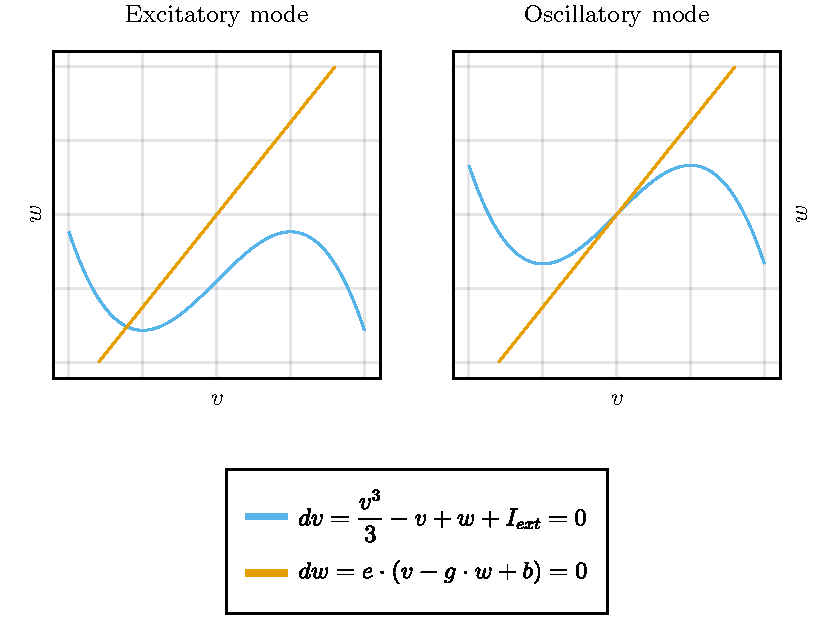
\includegraphics[height=8cm]{figures/fhn_dynamics/fhn_dynamics.pdf}
    \caption{The nullclines of the FitzHugh-Nagumo neuron.  Nullclines are isoclines where the derivative of a variable is zero.  Here we show an oscillatory mode and an excitable one.  In an oscillating cell, the stable equilibrium is replaced by an unstable equilibrium (open circle) around which it circles indefinitely.  See \citet{parsons2018} for a detailed explanation of the dynamics of oscillatory biological systems.}
\end{figure} % TODO: legend


\section{Simulation}

% Structure:
% - Describe the model, how the neurons are interconnected,
%   as well as how the model in general functions (as
%   a function which solves a system of ODEs)
% - Describe how the code works, in stages:
%    - Initialize parameters
%    - Integrate the solution to the system of DEs
%    - Simulate the muscle response using smoothing
%    - Construct the worm's shape using splines with the angle approach
%
% Basically, say enough that someone could replicate the idea without seeing the code at all.

We performed the simulations in Python, using the standard SciPy ODE solvers, which wrap LSODA, the Livermore Solver for Ordinary Differential Equations. % TODO list solver here

The main function of the code solves the FitzHugh-Nagumo equations of \Fref{eq: fhnd}, having one set of such equations per neuron, which is materialized from our CPG connectome, when given the state and a set of unchanging parameters.  This procedure is followed by the ODE solver which solves the trajectory of the system given some initial conditions; for example, if the neuron does not initially fire, the system may remain in a steady state and not oscillate.

\subsection{Overview of the methods}

We are outlining the code here, but the full code can be found at *** add clean github link here ***.

See the appendix, or attached code, for how we simulated this motion.  It will be published on Github with embedded plots, so people can see it.

We construct the network shown in \Fref{fig: cpg} with a system of ODEs, and solve it. The equations are integrated, giving a timeseries of neuronal potentials.  These were passed through filters to simulate muscular movement and the resistance of the medium.  We used Gaussian smoothing and B-splines for this purpose.
% TODO: reference for muscle response time

We generated a video by fixing the head of a worm to the origin, and re-normalizing the coordinates resulting from the filtering.

\subsection{Initializing the model's parameters}

% Mention that the FHN eqns are nondimensional and so all quantities have dimension but not units, i.e., arbitrary scaling.
We have used the FitzHugh-Nagumo equations for our model neurons; these equations are completely non-dimensional, meaning that their scaling is arbitrary.  As such, the constants, parameters, results, et cetera which we use have no units, and do not directly correspond to physical realities.

For a CPG model, each individual neuron has a set of parameters $\left\{α, γ, ε\right\}$ and each connection has a diffusion coefficient associated with it.  Additionally, it is easy to inject a current into a specific neuron, or to change a specific neuron's input requirements.

In short - each neuron in the CPG has two inputs from other neurons (the preceding neuron in the chain driving it, and the opposite neuron inhibiting it).

As such, there are five principal parameters per neuron: $α,\ γ,\ ε,\ D_\mathrm{desc},$ and $D_\mathrm{opp}$.  $D_\mathrm{desc}$ is the diffusion coefficient corresponding to the neuron directly before, and on the same side as, the ``current'' neuron.  Similarly, $D_\mathrm{opp}$ is the diffusion coefficient corresponding to the neuron on the opposite side of the nematode (dorsal or ventral).

These parameters are passed as an array to the function which solves the differential equation.  See ***Appendix A*** for parameter values which worked for us.

\subsection{Integrating the solution to the system of differential equations}

Integration is done by a standard differential equation solver.  To use the SciPy/LSODA interface, the function must take as input three objects $u,\ p,\ t$.  Here, $u$ is the current state of the system (the values of $v$ and $w$ for each neuron), $p$ is the set of parameters for the system (in our case, all $α,\ γ,\ ε,\ D_\mathrm{desc},$ and $D_\mathrm{opp}$ per neuron) and $t$ is the time (which we do not use, since our DEs do not depend on time).

The function must then return an array $du$, containing the derivatives $dv$ and $dw$ from each neuron.  In our program, we have structured this so that systems are grouped together, that is, the array looks like $\left[dv_1, dw_1, dv_2, dw_2, ..., dv_i, dw_i\right]$.

The function we have written is structured such that the parameters and state are ``unpacked'' from input arrays first, and then the equations are solved.

\subsection{Simulating the worm's muscular response}

The CPG network which we created is of the same form as the 2-D musculature of our simulated worm.  Each neuron is attached to a muscle; when it fires, it causes the attached muscle to contract.  We model the muscles as leaky integrators of the neuron's voltage. In this model, muscles can be seen as “leaky integrators” (Boyle et al. 2012) – the movement is heavily dependent on the current state of the neuron but is also dependent somewhat on the history. As a result, Gaussian smoothing of the neuron's voltage works to ``create'' an effective muscle contraction signal.  Through Gaussian smoothing, the movement is heavily dependent on the current state of the neuron but also dependent somewhat on the history.

Essentially, the process is that


\subsection{Constructing the worm's movement}

Much like \citet{izquierdo2018} did, we take a segment-based approach to the worm model.  Pairs of muscles on either side determine the overall angular displacement per segment.  The magnitude of the “contraction” resulting from the smoothing is interpreted as an angular displacement for that segment.  We use a cubic spline interpolation to smoothen the worm body.

Each neuron is assumed to be connected to a muscle; when it fires, it should cause that muscle to contract.
Pairs of neurons on either side determine the overall angular displacement per segment.
Gaussian smoothing and a cubic spline are used to mimic muscle movement and medium resistance.
The magnitude of the “contraction” resulting from the smoothing is interpreted as an angular displacement for that segment.


% TODO:
% - discuss dynamics of omega turn (central muscles contract in one direction,
%   extremities in another
% -

\subsection{Model versus Experimental Results}

Cite the paper which Jenny sent here.  It can be seen that our model closely approximates an unconstrained worm, specifically of the wild type.

While the angle which a worm crawling on agar subtends tends to be oblique, as the constraint on the worm decreases, the angle becomes more and more acute - consider the videos.  It can be seen that under the constraints of friction and other real-world conditions, the worm's range of motion is somewhat decreased.  If these constraints were removed, the muscles of the worm would be able to contract fully and thus produce behaviour much like our model does.  The worm undulates in a sinusoidal manner, both in simulation and reality.

\begin{figure}[h!]
    \centering
    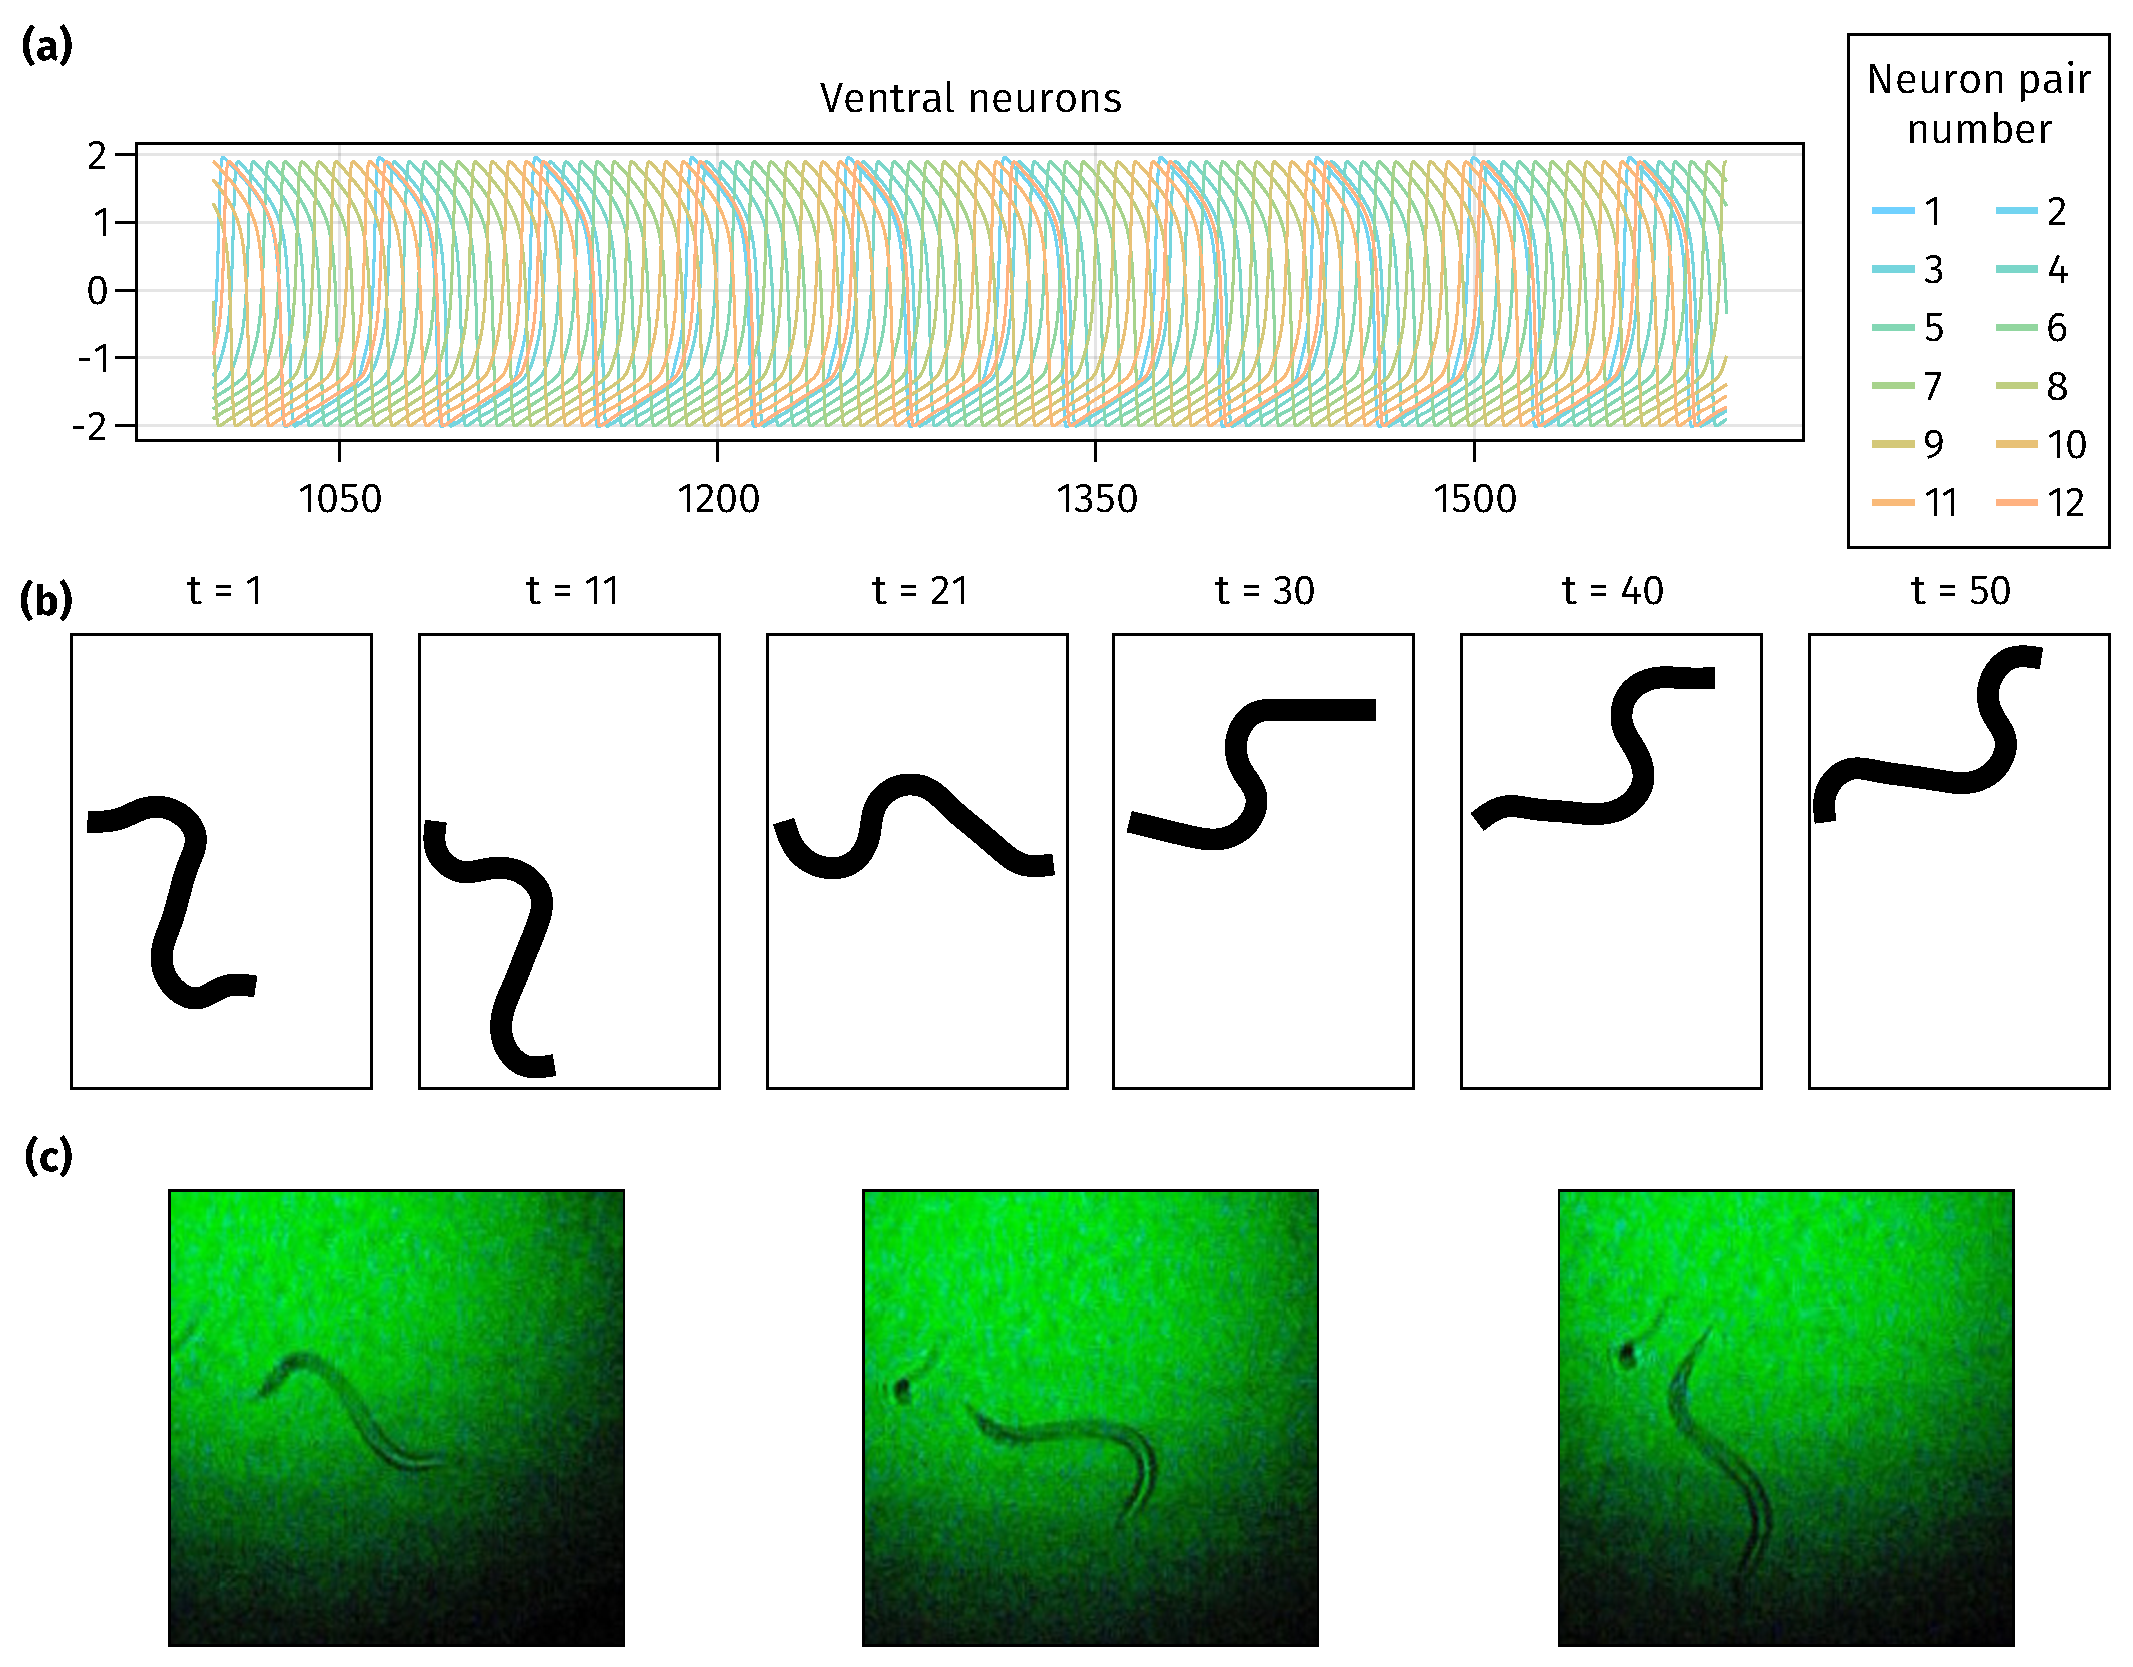
\includegraphics[height=13cm]{figures/worm_neuron_dash/worm_neuron_dash.pdf}
    \caption{A "dashboard view" representing the neuron and worm.  (a) shows the potentials of the ventral neurons, colored by number running down the worm.  (b) shows "images" of the simulated worm at different times. The worm was simulated by running the neuron potentials through a Gaussian filter to simulate muscle dampening, then taking the amplitude as an angular displacement, representing contraction or relaxation.  (c) shows images of a real \emph{C. elegans} in a cuvette, taken via shadow imaging.}
    \label{fig: worm_neuron_dash}
\end{figure}

% Closely related to the first I&B (2008).  Alternate and likely more realistic structure with a distributed CPG was proposed by new Izquierdo.

\section{Analog implementation}

\citet{nagumo1962} proposed a circuit to simulate a FitzHugh-Nagumo neuron, shown in \Fref{fig: nagumo_ckt}.  It used a tunnel diode to achieve a cubic-like activation function, and an inductor to differentiate the K current.  However, this approach presents several complications.  Tunnel diodes are rare, and rather expensive; inductors cannot be used in proximity because of mutual inductance effects, and are quite large.

\begin{figure}[h!]
    \centering
    \inputtikz{figures/nagumo/nagumo}
    \caption{The original circuit proposed by \citet{nagumo1962}.  Note the use of inductors for differentiation, and the tunnel diode to supply a cubic-like V-I curve.  Our circuit, based off \citet{keener1983}, is arranged in the same layout, to make the similarities and differences more explicit.}
    \label{fig: nagumo_ckt}
\end{figure}


The sodium channel in the FitzHugh-Nagumo equations has a negative resistance regime, wherein the current decreases as the voltage increases.  Nagumo's tunnel diode exhibits this behaviour, but it may be replaced by any device with a similarly nonlinear V-I curve.  The necessary feature consists of an oscillatory regime, the system is a relaxation oscillator, and that it has an excitable regime.

\citet{keener1983} proposed a modified Nagumo circuit which used the saturation properties of operational amplifiers ("op-amps") to achieve cubic-like non-linearity in the FHN model. He also used an op-amp and a capacitor to simulate the inductor in the original Nagumo circuit.

As a result of the piecewise linear approximation of the cubic, the nullclines of the circuit system differ slightly from the original FitzHugh-Nagumo nullclines.  However, in experiments this did not cause a significant change in the dynamics of the individual neuron, or many neurons connected together.  The nullclines are sufficiently similar that the dynamics are effectively the same.

Our modifications to Keener's proposed circuit are mainly concerned with diffusive coupling between neurons. If each individual circuit is thought of as a single neuron, then we implemented diffusive coupling methods between those neurons.  In that context, we found that you don't need separate power supplies, and you can get finer control by adjusting the bias voltage and input through a separate mechanism.

\begin{figure}[h!]
    \centering
    \inputtikz{figures/neuron_unit/neuron_unit}
    \caption{Our circuit, which is based of \citet{keener1983}.  Note the use of operational amplifiers in place of the inductor and tunnel diode; though this circuit might look more complex, in practice it is straight forward to implement.}
    \label{fig: neuron_unit}
\end{figure}

 In order to expand from a single neuron to a full central pattern generator, we implemented diffusive coupling mechanisms.  These mechanisms are shown in \Fref{fig: coupling}.  We implemented a positive diffusion coefficient by passing the voltage through a resistor (to simulate $D$, the diffusion coefficient), and then a diode (to simulate $\mathrm{max}(\Delta v, 0)$).  The negative diffusion coefficient was implemented by using an inverting amplifier with a small gain, and then passing through a diode.
\newsavebox{\tempbox}
\begin{figure}
    \centering
    \inputtikz{figures/coupling/coupling}
    \caption{Coupling methods}
    \label{fig: coupling}
\end{figure}

\subsection{Comparison of analog and simulation}

To compare the analog implementation with our simulated model, we will focus on the timeseries output of the neurons, and not on the end state worm.

\begin{figure}[h!]
    \centering
    \pgfplotsset{}
    % \inputtikz{figures/anal_sim_comp/anal_sim_comp}
    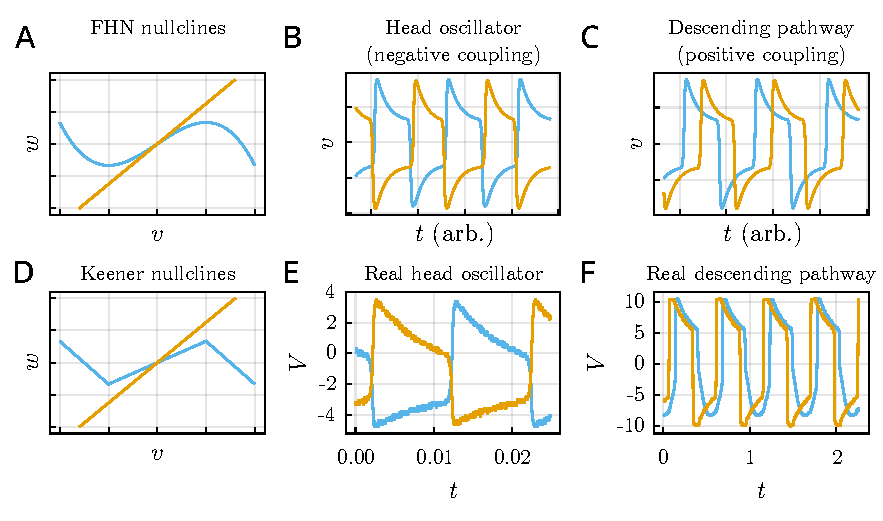
\includegraphics[height=9cm]{figures/anal_sim_comp/anal_sim_comp.pdf}
    \caption{Comparison between computationally simulated dynamics (top row) and observed dynamics in the analog circuit (bottom row).  (a) is the nullcline for the FitzHugh-Nagumo (simulated) equations, with the straight line being the $w$-nullcline and the cubic-like line being the $v$-nullcline; (b) is the "head oscillator" simulated (two neurons which mutually inhibit each other); (c) is the "descending pathway" simulated (one neuron driving another).  (d) is the nullcline for the analog circuit - a piecewise linear approximation to the cubic, (e) is the analog version of the head oscillator, and (f) is the analog version of the descending pathway.}
    \label{fig: anal_sim_comp}
\end{figure}

Looking at \Fref{fig: anal_sim_comp},

\subsection{Relevance of \citet{izquierdo2018} to our model}
% TODO: write up a section on the Beer paper and see how it relates to our CPG model.
% Perhaps a discussion about the "scientific lineage" of our model, and the Olivares et al model.
% Paraphrase their description.

The \citet{izquierdo2018} model is based on physical realities, and was generated using an evolutionary modelling process to find the structure of the descending neural network which controls muscular motion.  As a result, the model, while realistic, is complex, and differs from ours in several places.  First, the model is not a simple descending linked chain but a complex graphlike structure with repeating, complex self-oscillatory systems of neurons.

Our goal in modelling \emph{C. elegans} is not to produce a very physically accurate model, but rather to replicate those behaviours which are essential - and only those - to the movement of the nematode.  As such, we have the liberty of producing a simpler and more easily quantifiable model.

\section{Conclusion}

We have shown that the undulatory motion of \emph{C. elegans} can be simulated using a structured central pattern generator, and simple, biomimetic neurons.  This system is computationally cheap, and translates to a simple analog circuit.

Our model of the nematode is surprisingly similar to real unconstrained motion.  While most measurements of \emph{C. elegans} are taken on horizontal agar sheets, observations made in clear, water-filled cuvettes where the worm floats freely seem to resemble our simulated worm more.

Given the flexibility of the model, by introducing defects and asymmetries into the topology, we can study how mutations affect the nematode's motion, as well as the structures underlying differences in phenotypes.

% The particular model doesn't really matter; if you have the right topology, you can generate the behaviour.
% Reservoir computing and our neurons.  Speculate that different circuits of FHN neurons might be suitable dynamical reservoirs.  However, a CPG has a range of comparatively simple dynamics.
% cite Sanchez-Sinencio, Spano on circuits.  Theirs emphasize accuracy whereas ours emphasizes speed and minimal cost.

Reference some connections to \citet{adamatzky2008} - the neural system as a computational system.  Also cite similarity between B-Z and FHN.

\section{References}

% \nocite{*}
% \bibliography{References}
\printbibliography[heading=none]
\end{document}
